\section{Energiflöde genom väggar, burspråk och tak}

För att jämföra energiförluster genom en vägg med och utan isolering används
den tidigare beskrivna finita elementmetoden för värmeledningsekvationen i en dimension. Här approximeras
väggen som oändligt lång för enkelhet i beräkningarna. För alla beräkningar har ett tidssteg
på $\Delta t = \unit[500]{s}$ använts med semidiskret MOL.

\begin{figure}[hpbt]
\centering

\subfloat[\label{fig:tempdistapr}
Utomhustemperaturens variation en dag i april.]{
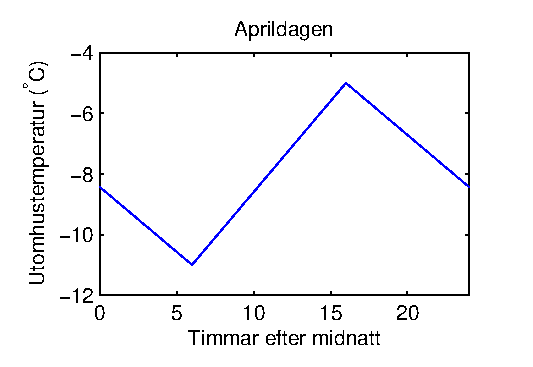
\includegraphics[width=6cm]{images/temperatureapr.eps}}\vspace{1cm}
\subfloat[\label{fig:tempdistdec}
Utomhustemperaturens variation en dag i december.]{
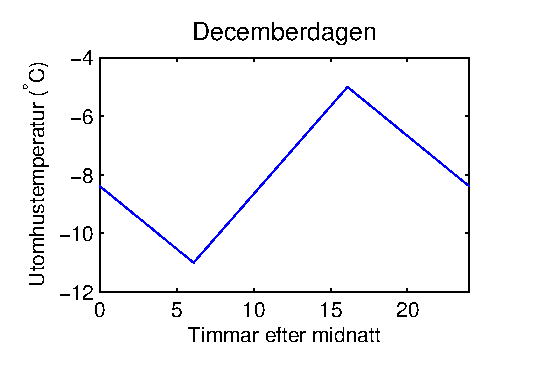
\includegraphics[width=6cm]{images/temperaturedec.eps}
}

\caption{\label{fig:temperaturedist} Utomhustemperaturens variation under standarddagarna motsvarande mitten av april samt den sista december som varierar mellan $\unit[6]{^\circ C}$ på natten och $\unit[9]{^\circ C}$ på dagen respektive $\unit[-11]{^\circ C}$ på natten och $\unit[-5]{^\circ C}$ på dagen.
}
\end{figure}

I detta försök antas att en perfekt värmeanläggning
existerar så att temperaturen inomhus hålls till konstant $\unit[20]{^\circ C}$. Efter detta specificeras energiflödet
från utsidan av väggen genom vilka energiflöden som strömmar till väggen. Dessa är svartkroppsstrålning, solinstrålning
samt konvektion. Beräkningarna är sedan genomförda med solinstrålningsdata från en solig och en molnig december samt
en solig och en molnig aprildag. Solens position och mängden svartkroppsstrålning är beräknade enligt avsnitt \ref{sec:blackbody} och
\ref{sec:sunthroughwindows}. Enligt detta recept kan nu neumannvillkoret
på utsidan av väggen tecknas som ekvation~\eqref{eq:wallneumann}. Här är $T_{ref}$ utomhustemperaturen
och $\partial T/\partial n$ betecknar normalderivatan.

\begin{equation}
\label{eq:wallneumann}
\frac{1}{k}\frac{\partial T}{\partial n} = Q_{sol} + Q_{svartkropp} + h(T_{ref}-T)
\end{equation}

Konvektionsparametern och temperaturen under april- respektive decemberdagen har satts till värden som kan ses i tabell~\ref{tbl:aprdec}. Temperaturen har sedan linjariserats mellan dessa värden över dagen, vilket kan ses i figur~\ref{fig:temperaturedist}. Att sätta temperaturvariationen till en triangelvåg med maximalt och minimalt värde vid samma tidpunkt i både april och december är en approximation av hur det ofta blir när vädret är relativt konstant över flera dagar. Vädret skiftar dock hela tiden och den faktiska utomhustemperaturen är relativt godtycklig.

\begin{table}[hpbt]
\centering
\caption{Data som använts för vindstilla aprildag respektive blåsig decemberdag.}
\begin{tabular}{c|c|c}
& April & December \\
\hline
Vind parallell mot väggen [$ms^{-1}$] & 0 & 7 \\
Motsvarande h-värde [$Wm^{-2}K^{-1}$] & 6,19 & 35 \\
Temperatur kl 06 [$^{\circ}C$] & 6 & -11 \\
Temperatur kl 16 [$^{\circ}C$] & 9 & -5
\end{tabular}
\label{tbl:aprdec}
\end{table}


Problemet har sedan satts upp för två olika väggar, en som enbart innehåller $\unit[0,5]{m}$ tegel, och en som innehåller samma tegellager men som dessutom har tilläggsisolerats på utsidan med $\unit[0,1]{m}$ mineralull. Materialkonstanterna för aktuella ämnen kan ses i tabell~\ref{tbl:materialconstants}.

\begin{table}[hpbt]
\centering
\caption{Använda materialkonstanter, hämtade från referens \cite{kandidatarbete2010}, \cite{engineeringtoolboxdensity}, \cite{bkvthermal}, \cite{engineeringtoolboxspecificheat}, \cite{engineeringcom}, \cite{engineeringtoolboxthermalconductivity} och \cite{ozel11}. $k$ betecknar här värmelednningsförmågan, medan $c_p\rho$ anger volymetriska värmekapacitiviteten.}
\begin{tabular}{c|c|c|c|c|c|c}
& Tegel & Mineralull & Koppar & Spånskiva & Puts & Takpannor \\
\hline
$k$ [$Wm^{-1}K^{-1}$] & 0,6 & $5,2\cdot 10^{-7}$ & 401 & 0,5 & 0,25 & 0,85\\
$c_p \rho$ [$kJ~m^{-3}$] & 1154 & 58,8 & 3490 & 1300 & 872 & 1748
\end{tabular}
\label{tbl:materialconstants}
\end{table}

Under experimentens gång  har ett godtyckligt initialvärde valts för att sedan vänta tills
lösningen stabiliserat sig för att då utläsa energiåtgången. Derivatan på insidan har slutligen beräknats
och använts för att beräkna kyleffekten genom Fouriers värmelag.

För burspråk och tak har ungefär samma metod som för väggen följts, med fyra simuleringar motsvarande soliga och
molniga december- och aprildagar. Samma temperaturförändringar som beskrivits ovan har använts för
respektive fall. Skillnaderna ligger i vilka material de olika byggnadsdelarna är uppbyggda av.
Burspråket har simulerats med materialen och tjocklekarna angivna för burspråken i figur~\ref{fig:bursprak} och tillhörande konstanter från tabell~\ref{tbl:materialconstants}.

Taket är uppbyggt enligt figur~\ref{fig:taket} och består av omkring tre centimeter tegelpannor och 21 centimeter mineralull. Den högst marginella påverkan som gipset medför har försummats. Övriga skillnader mellan beräkningar på värmeflödet genom taket och väggarna härstammar från det faktum att solstrålningens normalprojektion är annorlunda på taket jämfört med vertikala ytor, något som har tagits med i beräkningarna. Dessutom blir denna projektion olika beroende på om man betraktar nordsidan eller sydsidan av taket, varför dessa två delar har simulerats separat för de soliga dagarna. De molniga dagarna har det däremot antagits att en femtedel av den maximala solintensiteten infaller på samtliga ytor, då all strålning kan antas vara indirekt.

Vidare har väggarnas stegsvar undersökts. Först var väggarna i jämvikt med en utomhustemperatur på $T = \unit[0]{^\circ C}$ som sedan steg till $T = \unit[10]{^\circ C}$ vid tiden $t=0$. Konvektionsparametern är här satt till
$h = \unit[25]{W~m^{-2}~K^{-1}}$ vilket motsvarar en vind på ungefär 
$v = \unit[5]{m~s^{-1}}$ parallellt med väggens yta. Genom att beräkna den momentana kyleffekten för varje tidssteg kunde väggarnas tröghet studeras.
